% Barrowmaze Session Form
% Copyright (c) 2022-2023 Peter H. Froehlich <peter.hans.froehlich@gmail.com>.
% License terms: CC BY-SA 4.0

\section{Barrowmaze Session Form}
\label{sessionform}
I use this form to track the two-hour Barrowmaze sessions I run.
I print them two to a page, four to a sheet. So what's what here?

\textbf{Date:}
%
Literally just the date of the session.
%
In our game ``campaign time'' is the same as ``real time'' so there's usually
no confusion.

\textbf{Players:}
%
Names of the (up to) three players in ``initiative order'' for their side.
%
I have players roll a d6 \emph{ahead of time} as often as necessary to get them
into a linear order for the session; less rolling during combats and less chaos.
%
In the very rare case that there's a fourth player, I just squeeze them in
somehow.

\textbf{Turn Tracker:}
%
Each box represents a ten-minute game turn and I've never needed more than
eight hours total.
%
At the top, every \emph{other} column is marked \monster{} for random encounter
checks; at the bottom, every \emph{sixth} column is marked, the first three
\torch{} because torches would burn out then, the final one \lantern{} because
both torches and lanterns would burn out then.

I roll eight hours worth of random encounters ahead of time and fill in the
turns in which they will happen with red pencil; that way I can foreshadow an
encounter if appropriate; other ``pre-rolled random-ish events'' can be marked
using a second (or third) color.

% use 270 if it's an odd page instead?
% I hate tables facing west :D
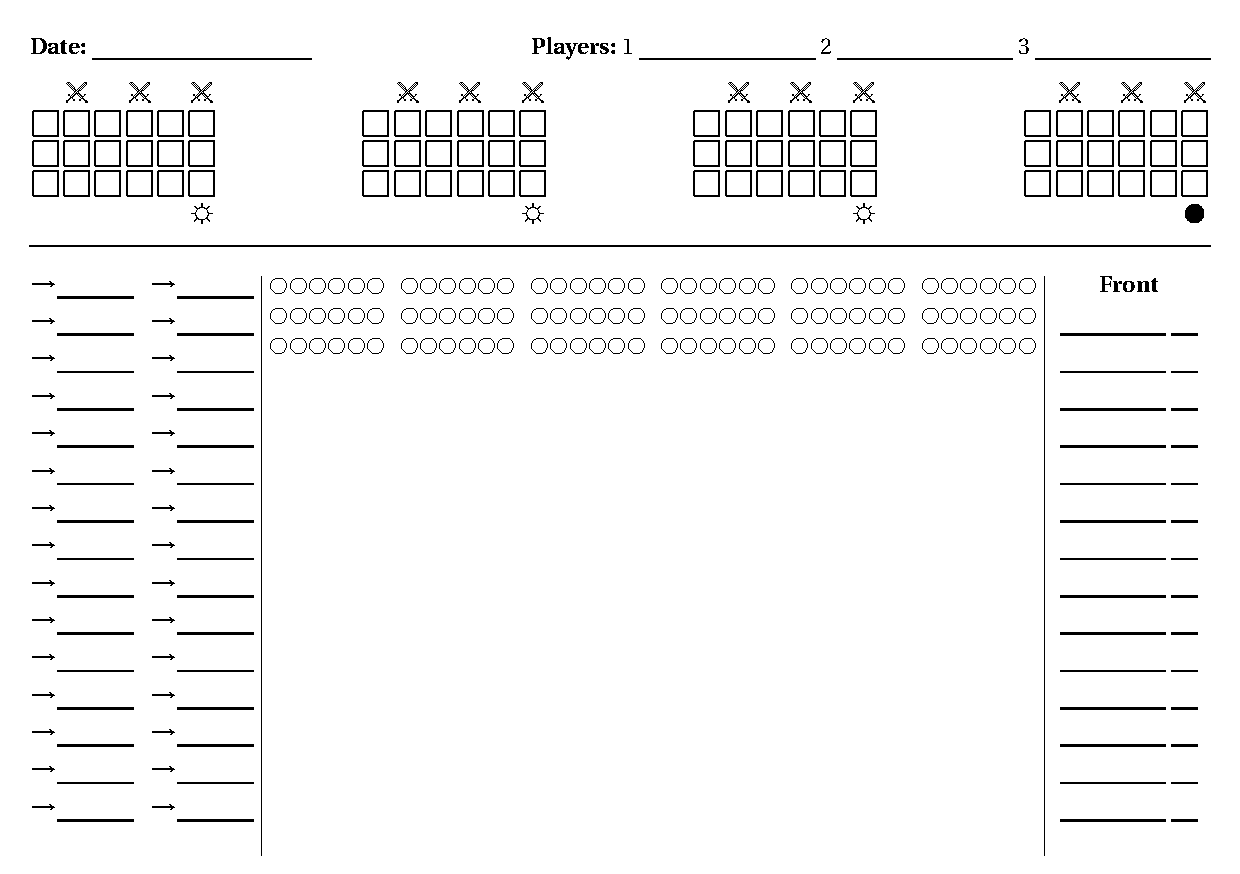
\includepdf[angle=90]{vendor/session-form.pdf}

\textbf{Room Numbers:}
%
The left-hand column is used to track the party's route through the dungeon;
this is mostly useful \emph{after} the session when it comes to restocking.
%
I only make ``restock rolls'' for rooms the party \emph{saw empty}, not for all
rooms that in fact \emph{are empty}.

\textbf{Marching Order:}
%
The right-hand column has the party's \emph{marching order} including who
carries what kind of \emph{light source} (L = lamp, T = torch, M = magic); I
encourage single-file simply because it means fewer PCs falling into bottomless
pits, but I am flexible if players \emph{insist} on walking next to each other
(I just put a line next to ``pairs'' on the far right).

\textbf{Random Notes:}
%
The middle column is for free-form notes of \emph{any} kind; I usually track
hit points of monsters there, but also reminders of treasures found and other
changes the party made to the dungeon.
%
There is also a \emph{round tracker} but I only use it when I have to, for
example because a monster they just killed will get up again or because a
character only has a few rounds left to live.
\by{phf}
\endinput
